%%%%%%%%%%%%%%%%%%%%%%%%
%% Sample use of the infthesis class to prepare a thesis. This can be used as 
%% a template to produce your own thesis.
%%
%% The title, abstract and so on are taken from Martin Reddy's csthesis class
%% documentation.
%%
%% MEF, October 2002
%%%%%%%%%%%%%%%%%%%%%%%%

%%%%
%% Load the class. Put any options that you want here (see the documentation
%% for the list of options). The following are samples for each type of
%% thesis:
%%
%% Note: you can also specify any of the following options:
%%  logo: put a University of Edinburgh logo onto the title page
%%  frontabs: put the abstract onto the title page
%%  deptreport: produce a title page that fits into a Computer Science
%%      departmental cover [not sure if this actually works]
%%  singlespacing, fullspacing, doublespacing: choose line spacing
%%  oneside, twoside: specify a one-sided or two-sided thesis
%%  10pt, 11pt, 12pt: choose a font size
%%  centrechapter, leftchapter, rightchapter: alignment of chapter headings
%%  sansheadings, normalheadings: headings and captions in sans-serif
%%      (default) or in the same font as the rest of the thesis
%%  [no]listsintoc: put list of figures/tables in table of contents (default:
%%      not)
%%  romanprepages, plainprepages: number the preliminary pages with Roman
%%      numerals (default) or consecutively with the rest of the thesis
%%  parskip: don't indent paragraphs, put a blank line between instead
%%  abbrevs: define a list of useful abbreviations (see documentation)
%%  draft: produce a single-spaced, double-sided thesis with narrow margins
%%
%% For a PhD thesis -- you must also specify a research institute:
%\documentclass[phd,ilcc,twoside]{infthesis}

%% For an MPhil thesis -- also needs an institute
% \documentclass[mphil,ianc]{infthesis}

%% MSc by Research, which also needs an institute
% \documentclass[mscres,irr]{infthesis}

%% Taught MSc -- specify a particular degree instead. If none is specified,
%% "MSc in Informatics" is used.
\documentclass[msc,ai]{infthesis}
%\documentclass[msc]{infthesis}  % for the MSc in Informatics

%% Master of Informatics (5 year degree)
% \documentclass[minf]{infthesis}

%% Undergraduate project -- specify the degree course and project type
%% separately
% \documentclass[bsc]{infthesis}
% \course{Artificial Intelligence and Psychology}
% \project{Fourth Year Project Report}

%% Put any \usepackage commands you want to use right here; the following is 
%% an example:
%\usepackage[number]{natbib}
\usepackage[natbibapa]{apacite}
\usepackage{parskip}
\usepackage{graphicx}
\usepackage{caption}
\usepackage{float}
\usepackage{amsmath}
\usepackage{subfig}
\usepackage{kpfonts}



% figures' path
\graphicspath{{figures/}}

\setlength{\parindent}{0cm}
%% Information about the title, etc.
\title{How I Did It}
\author{Victor von Frankenstein}

%% If the year of submission is not the current year, uncomment this line and 
%% specify it here:
% \submityear{1785}

%% Optionally, specify the graduation month and year:
% \graduationdate{February 1786}

%% Specify the abstract here.
\abstract{%
    This doctoral thesis will present the results of my work into the
    reanimation of lifeless human tissues.
}

%% Now we start with the actual document.
\begin{document}

%% First, the preliminary pages
\begin{preliminary}

%% This creates the title page
\maketitle

%% Acknowledgements
\begin{acknowledgements}
Many thanks to my mummy for the numerous packed lunches; and of course to
Igor, my faithful lab assistant.
\end{acknowledgements}

%% Next we need to have the declaration.
\standarddeclaration

%% Finally, a dedication (this is optional -- uncomment the following line if
%% you want one).
% \dedication{To my mummy.}

%% Create the table of contents
\tableofcontents

%% If you want a list of figures or tables, uncomment the appropriate line(s)
% \listoffigures
% \listoftables

\end{preliminary}

%%%%%%%%
%% Include your chapter files here. See the sample chapter file for the basic
%% format.

\chapter{Introduction}
\label{chap:introduction}

In this chapter, we will first briefly introduce the Recurrent Neural Network (RNN) and the branch prediction, which reflect the motivation of this project. Then we will discuss the objectives and contribution of the project. Finally, we also describe the structure of this document.

\section{Motivation of the Project}
\label{sec:motivation}

In the area of Machine Learning, RNN is a type of neural network, which is good at capturing the tenporal features of sequential data. Therefore, RNN is widely used to predict and label sequential data in the area of Natural Language Processing(NLP), for example recognising sequential speech data ~\citep{graves2013speech} and language modeling ~\citep{mikolov2010recurrent}. Specifically, different types of RNN were used in these works, the most popular types are the Long Short-Term Memory network (LSTM) ~\citep{gers1999learning}, bidirectional RNN ~\citep{graves2013speech} and the Gated Recurrent Unit network (GRU) ~\citep{cho2014learning}. 

Furthermore, a branch predictor predicts the direction of a branch given the program history. A mispredicted branch could cause the waste of program work ~\citep{michaud1996skewed}. Therefore, it is important to improve the accuracy of the branch prediction. A higher prediction accuracy could offset the misprediction penalties and improve the performance of the processor ~\citep{leedynamic}. The state-of-the-art branch predictor uses the partial matching compression algorithm and achieves the accuracy of 99\% ~\citep{seznec2006case}.

Finally, because program branches are time-based, branch prediction could benefit from the usage of RNN. This project aims at predicting branch outcomes given the branch history using RNN. The primary purpose of this project is to build the RNN branch predictor, which is a new attempt in the area of branch prediction. Moreover, to make the RNN predictor more competitive with the state-of-the-art brach predictors, different RNN types and ML techniques are used, which will be described in subsequent chapters. 

\section{Objective and Contribution of the Project}
\label{sec:objective}

The primary objective of the project is to build an RNN branch predictor, which could predict the future outcome of a branch given the branch history. More specifically, instead of building a predictor whose performance exceeds the existing best predictor, we focus on attempting different techniques in ML and find a relatively better model configuration. Besides, the second objective is exploring the influence of varying branch history length, and various training set size has on the model's performance.

Our contributions could be...

\section{Structure of the Dissertation}
\label{sec:structure}
\chapter{Background}
\label{chap:background}
In this chapter, we will provide the basic knowledge of the techniques used in this project, including the RNN, the branch prediction, the dataset, and the methods used during training. We will first present the basic concept of each technique, and then the relevant literature will be provided.

\section{Recurrent Neural Network}
\label{sec:rnn}
\subsection{Basic Knowledge}
\label{sec:bk_rnn}
RNN is a type of neural network, different from the feed-forward neural network, RNN could remember the information from the previous input data, which benefits from the recurrent pattern inside the RNN units. Figure ~\ref{fig:unrolled} shows the structure of the vanilla RNN and the unrolling version. We could see that the output $o_t$ depends on both the input at time $t$ ($x_t$) and the previous hidden state $s_{t-1}$. The output at time $t$ could be calculated by the euations below, where $f$ could be a nonlinear function.

\begin{equation}
\begin{aligned}
s_t = f(Ux_t + Ws_{t-1})\\ 
o_t = softmax(Vs_t)
\label{eq:rnn}
\end{aligned}
\end{equation}

\begin{figure}[H]
\centering
\captionsetup{justification=centering,margin=1cm}
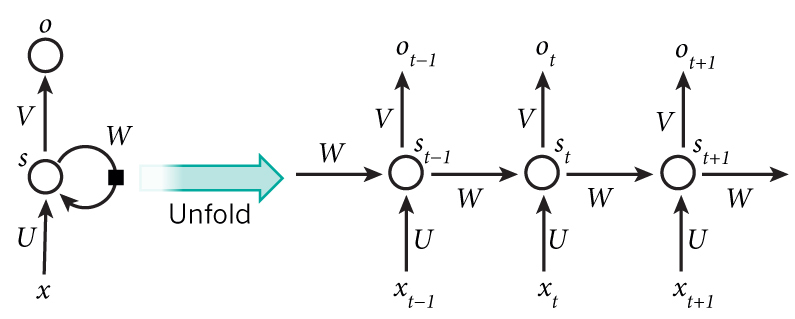
\includegraphics[width=\textwidth]{rnn.jpg}
\caption{Unrolling an RNN unit. Left is the original RNN, right is the unrolled version. $x_t$ is the input at time $t$, $s_t$ is the hidden state of the RNN at time $t$, $o_t$ is the output of the RNN at time $t$. $W$ and $V$ are the weight matrix.}
\caption*{Source: http://www.wildml.com/2015/09/recurrent-neural-networks-tutorial-part-1-introduction-to-rnns/}
\label{fig:unrolled}
\end{figure}

There are three popular types of RNN units, including the vanilla RNN, the LSTM ~\citep{hochreiter1997long}, and the GRU ~\citep{cho2014learning}. The main difference among these three types of RNNs is the choice of the function $f$ in the Equation \ref{eq:rnn}. As shown in Figure \ref{fig:rnn_units}, in the vanilla RNN unit, the $f$ is a simple $tanh$ function. While, in the LSTM and GRU, the $f$ is a combination of several functions. The complex structures inside the LSTM and GRU unit could solve the long-term dependency problems caused by the simple $tanh$ function in the vanilla RNN unit ~\citep{hochreiter1997long}.

\begin{figure}[H]
\centering
\subfloat[Vanilla RNN unit.]{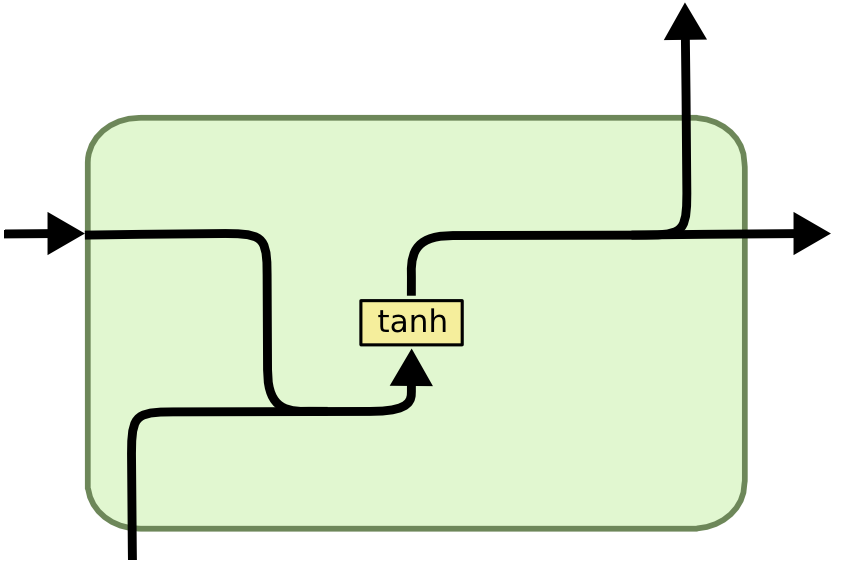
\includegraphics[width=.33\textwidth]{rnn_unit.png}}
\subfloat[LSTM unit.]{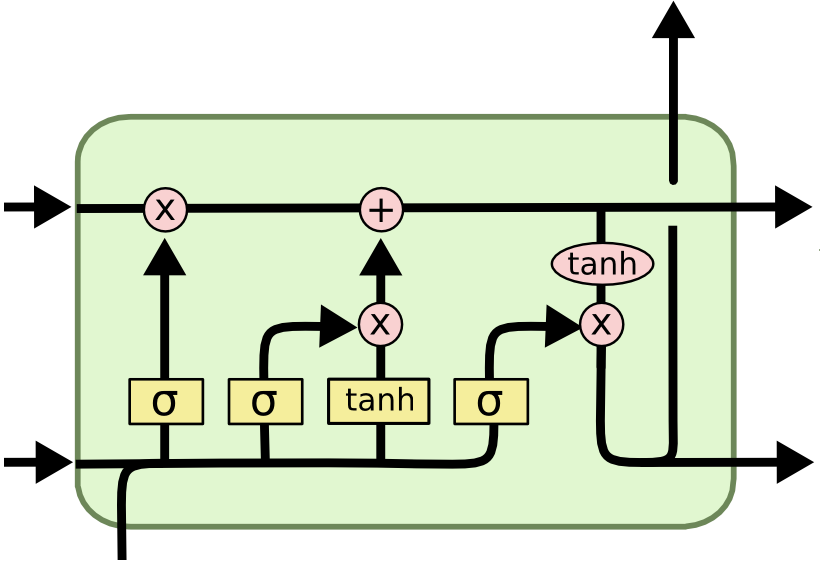
\includegraphics[width=.33\textwidth]{lstm_unit.png}}
\subfloat[GRU unit.]{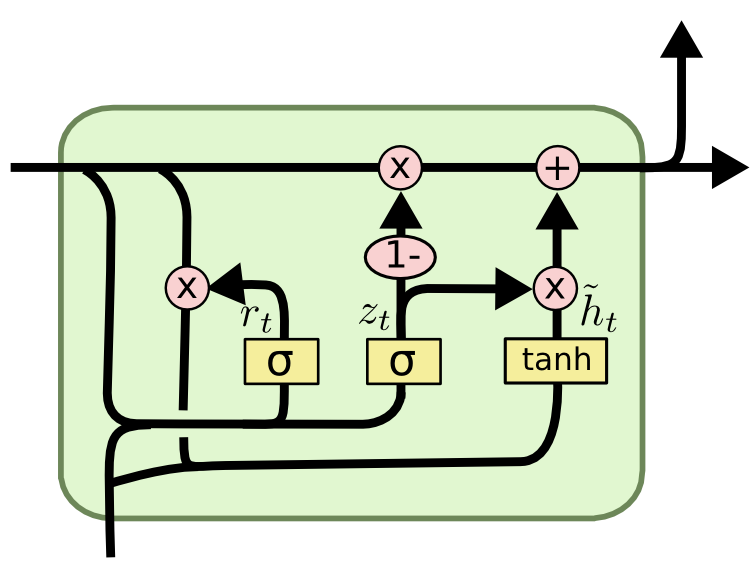
\includegraphics[width=.33\textwidth]{gru_unit.png}}
\caption{Three types of RNN units.}
\caption*{Source: http://colah.github.io/posts/2015-08-Understanding-LSTMs/}
\label{fig:rnn_units}
\end{figure}

Bidirectional RNNs are similar to the 2-layered RNNs, except that the first RNN layer receives the input sequence word by work from left to right, while the second layer gets the input sequence from right to left ~\citep{schuster1997bidirectional}. Therefore, bidirectional RNNs could capture the information before and after the current input data. The RNN unit inside the bidirectional RNNs could be the vanilla RNN unit, the LSTM unit, or the GRU. Figure \ref{fig:birnn} shows a basic bidirectional RNN, we could see that the output $y_t$ is computed based on the concatenation of forward and backward hidden states in the RNN.

\begin{figure}[H]
\centering
\captionsetup{justification=centering,margin=1cm}
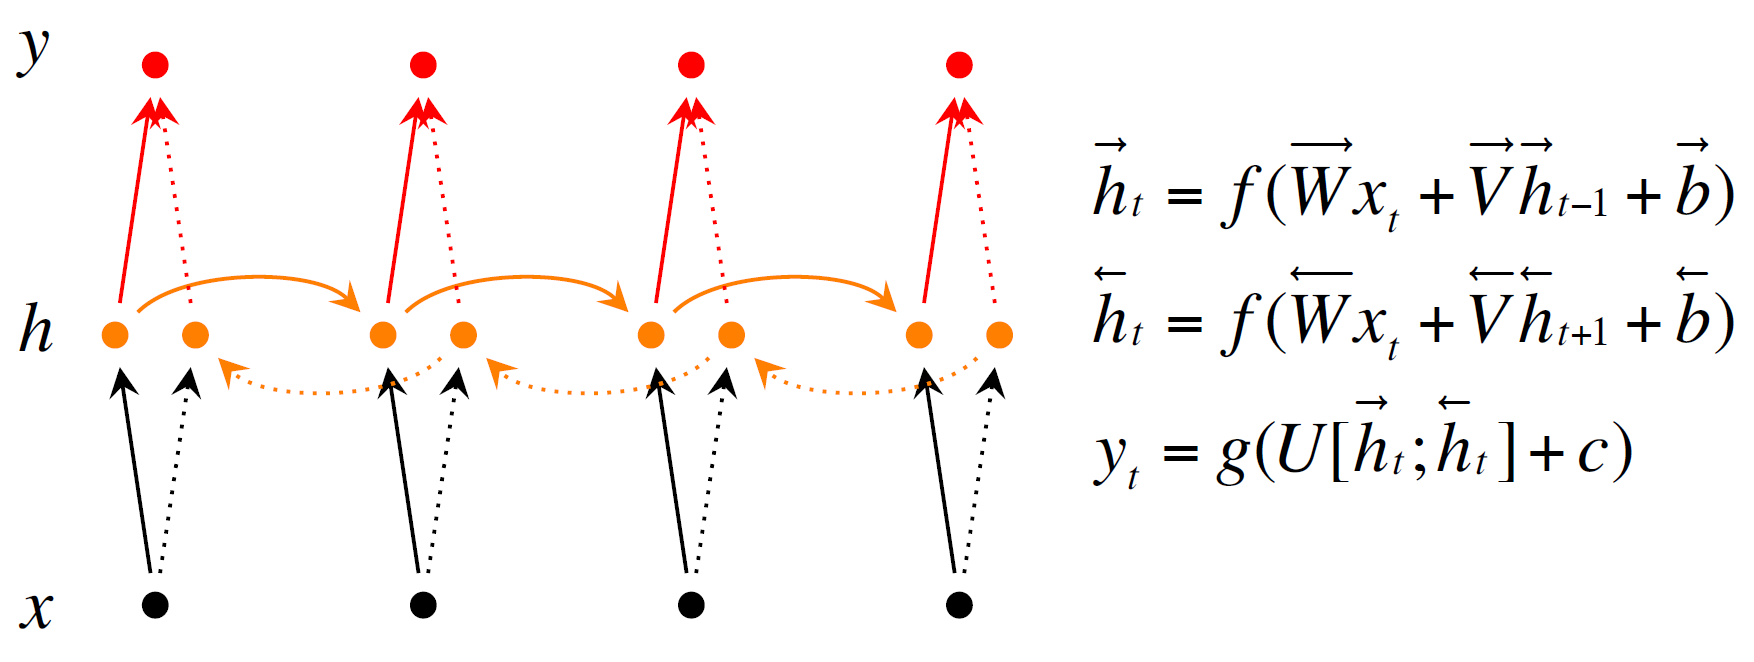
\includegraphics[width=\textwidth]{birnn.png}
\caption{The bidirectional RNN. $\protect\overrightarrow{h_t}$ is the forward RNN hidden state,  $\protect\overleftarrow{h_t}$ is the backward RNN hidden state. $x_t$ is the input at time $t$, $y_t$ is the output at time $t$. $f$ is the function inside the unit, which could be the vanilla RNN, LSTM, and GRU.}
\caption*{Source: http://web.stanford.edu/class/cs224n/lectures/lecture9.pdf}
\label{fig:birnn}
\end{figure}

attention

\subsection{Relevant Literature}
\label{sec:rl_rnn}

\section{Branch Prediction}
\label{sec:bp}

\subsection{Basic Knowledge}
\label{sec:bk_bp}

\subsection{Relevant Literature}
\label{sec:rl_bp}

\section{Dataset}
\label{sec:dataset}
Introduce the branch prediction championship competition and the related dataset.

\section{Training Procedure}
\label{training}
This part introduce the metrics used during training, like dropout, adam optimization, learning rate ...



\chapter{Inplementation}
\label{chap:inplementation}
 
In this chapter, we will provide the experimental inlementation in details, including the data processing, the default architecture of the model, and the detailed experimental design.
 
\section{Data Preprocess}
\label{preprocess}

\section{Model Architecture}
\label{architecture}

\section{Experiment Design}
We designed four group of experiments. In each group, we fixed the 
\label{setup}

\subsection{Varying History Length}
\label{history}

\subsection{Varying Training Set Size}
\label{training_size}

\subsection{Varying Network Types}
\label{network_type}

\subsection{Hyperparameters}
\label{hyperparameters}




\chapter{Results}
\label{chap:results}
In this chapter, we will show the experiment results of different models. We evaluate the performance of the models based on the prediction accuraccy on the test set. We fixed the parameters and change the key variables in each group of experiments.
 
\section{Results Based on Different History Size}
\label{results_history}

\section{Results Based on Different Training Set Size}
\label{results_size}

\section{Results Based on Different Network Type}
\label{results_type}

\section{Results after Parameter Optimization}
\label{resullts_para}



% \include{chap2}
%% ... etc ...

%%%%%%%%
%% Any appendices should go here. The appendix files should look just like the
%% chapter files.
\appendix
\include{appendix1}
%% ... etc...

%% Choose your favourite bibliography style here.
%\bibliographystyle{apalike}
\bibliographystyle{apacite}

%% If you want the bibliography single-spaced (which is allowed), uncomment
%% the next line.
% \singlespace

%% Specify the bibliography file. Default is thesis.bib.
\bibliography{reference}

%% ... that's all, folks!
\end{document}
